\documentclass[12pt, a4paper,hyperref]{article} % 必須使用Xelatex編譯
%\usepackage{ctex}
\usepackage[margin=3cm]{geometry}
\usepackage{amsmath,amsthm,amssymb} % 引入 AMS 數學環境
\usepackage{hyperref} % 生成書籤
\usepackage{bookmark} % 書籤加強版
\usepackage{xeCJK} % 中文
\usepackage{zhnumber}%中文編號
\usepackage{yhmath} % math symbol
\usepackage{graphicx} % 圖形插入用
%\usepackage{wrapfig} % 文繞圖
\usepackage{fontspec}    % 加這個就可以設定字體
\usepackage{type1cm}	 % 設定fontsize用
\usepackage{titlesec}   % 設定section等的字體
\usepackage{titling}    % 加強 title 功能
\usepackage{fancyhdr}   % 頁首頁尾
\usepackage{tabularx}   % 加強版 table
\usepackage{booktabs}    %三線表靠它了	
\usepackage{multirow}
\usepackage{diagbox}
\usepackage[square, comma, numbers, super, sort&compress]{natbib}  % cite加強版
\usepackage[usenames, dvipsnames]{color}  % 可以使用顏色\color{red}
\usepackage{enumerate}  % 標號
\usepackage{enumitem} % 標號
\usepackage[normalem]{ulem} % 刪除線\sout{}
\usepackage{cancel}
\usepackage{indentfirst}
\usepackage{bbm}
\usepackage{pifont}
\usepackage{prettyref} % 放超連結\label{}\prettyref{}
\usepackage{multicol} % 局部分欄
\usepackage{float}  % 浮動環境
\usepackage{subfigure} % 並排圖片
\usepackage{verbatim}  % 大註解
\usepackage[version=4]{mhchem} % 化學模式\ce{[AgCl2]-}
\usepackage{chemfig} % 化學結構
\usepackage{listings} % 清單
\usepackage{xcolor} % 可以定義色彩


\usepackage{sectsty} %section 格式
\usepackage{type1cm} %字體大小
\usepackage{indentfirst} %首行縮排
\usepackage{fontspec}                  %引入字体设置宏包
\setmainfont{Times New Roman}


%%%%%%%%%%%%%%中文 Environment%%%%%%%%%%%%%%%
\setCJKmainfont{AR PL KaitiM Big5}
\setCJKsansfont{AR PL KaitiM Big5}
\setCJKmonofont{AR PL KaitiM Big5}
\defaultCJKfontfeatures{AutoFakeBold=6,AutoFakeSlant=.4} %以後不用再設定粗斜
\newCJKfontfamily\Kai{標楷體}
\newCJKfontfamily\Hei{微軟正黑體}
\newCJKfontfamily\NewMing{新細明體}
\setCJKmainfont[AutoFakeBold=3,AutoFakeSlant=.4]{標楷體}%中文字分開設定字體
\XeTeXlinebreaklocale "zh"             %這兩行一定要加,中文才能自動換行
\XeTeXlinebreakskip = 0pt plus 1pt     %這兩行一定要加,中文才能自動換行


%%%%%%%%%%%%%%%頁面設定%%%%%%%%%%%%%%%
\setlength{\headheight}{15pt}  %with titling
\setlength{\droptitle}{-1.5cm} %title 與上緣的間距
\parindent=24pt %設定縮排的距離
%\parskip=1ex  %設定行距
%\pagestyle{empty}  % empty: 無頁碼
%\pagestyle{fancy}  % fancy: fancyhdr

%use with fancygdr
%\lhead{\leftmark}
%\chead{}
%\rhead{}
%\lfoot{}
%\cfoot{}
%\rfoot{\thepage}
%\renewcommand{\headrulewidth}{0.4pt}
%\renewcommand{\footrulewidth}{0.4pt}

%\fancypagestyle{firststyle}
%{
  %\fancyhf{}
  %\fancyfoot[C]{\footnotesize Page \thepage\ of \pageref{LastPage}}
  %\renewcommand{\headrule}{\rule{\textwidth}{\headrulewidth}}
%}

%%%%%%%%%%%%%% 自定義Style%%%%%%%%%%%%%%
\newtheoremstyle{mystyle}
  {6pt}{15pt}%       上下間距
  {}%               內文字體
  {}%               縮排
  {\bf}%            標頭字體
  {.}%              標頭後標點
  {1em}%            內文與標頭距離
  {}%               Theorem head spec (can be left empty, meaning 'normal')

% 改用粗體,預設 remark style 是斜體
\theoremstyle{mystyle}	% 定理環境Style

%%%%%%%%%%%%%%code Environment%%%%%%%%%%%%%%%
\definecolor{commentgreen}{RGB}{2,112,10}
\definecolor{eminence}{RGB}{108,48,130}
\definecolor{weborange}{RGB}{255,165,0}
\definecolor{frenchplum}{RGB}{129,20,83}

%%%%%url%%%%%
\usepackage{url}%網址會亮
\def\UrlBreaks{\do\A\do\B\do\C\do\D\do\E\do\F\do\G\do\H\do\I\do\J
\do\K\do\L\do\M\do\N\do\O\do\P\do\Q\do\R\do\S\do\T\do\U\do\V
\do\W\do\X\do\Y\do\Z\do\[\do\\\do\]\do\^\do\_\do\`\do\a\do\b
\do\c\do\d\do\e\do\f\do\g\do\h\do\i\do\j\do\k\do\l\do\m\do\n
\do\o\do\p\do\q\do\r\do\s\do\t\do\u\do\v\do\w\do\x\do\y\do\z
\do\.\do\@\do\\\do\/\do\!\do\_\do\|\do\;\do\>\do\]\do\)\do\,
\do\?\do\'\do+\do\=\do\#}%URL断行
%%%%%%%%%%%%%% new commands: %%%%%%%%%%%%%%
\newcommand{\np}[1]{\\[{#1}] \indent}
\newcommand{\transpose}[1]{{#1}^\mathrm{T}}
\newcommand{\adj}{\mathrm{adj}}
\newcommand{\degree}{^\circ}
\newcommand{\Arc}[1]{\wideparen{{#1}}}
\newcommand{\sline}[1]{\overleftrightarrow{{#1}}}
\newcommand{\Ray}[1]{\overrightarrow{{#1}}}
\newcommand{\Segment}[1]{\overline{{#1}}}
\renewcommand{\proofname}{\bf 證明:} 
\newcommand{\pole}[2]{\mathbb{P}_{\mathcal{#1}} (#2)}
\newcommand{\tg}[2]{\mathcal{T}_{\mathcal{#1}} (#2)}
\newcommand{\mul}{\ce{\mu l}}
\newcommand{\mug}{\ce{\mu g}}
\newcommand{\upcite}[1]{\textsuperscript{\cite{#1}}} %参考文献上标
%%%%%%%%%%%%%%計數器%%%%%%%%%%%%%%%
\newtheorem{ans}{Answer}[section] %答案
\newtheorem{ax}{Axiom}[section] %公理
\newtheorem{cl}{Corollary}[section] %推論
\newtheorem{con}{Conclusion}[section] %結論
\newtheorem{clm}{Claim}[section] %主張,聲稱
\newtheorem{df}{Definition}[section] %定義
\newtheorem{ex}{Example}[section] %例題
\newtheorem{exs}{Exercise}[section] %習題
\newtheorem{lm}{Lemma}[section] %引理
\newtheorem{pr}{Problem} %問題
\newtheorem{pf}{Proof}[section] %證明
\newtheorem{pro}{Property}[section] %性質
\newtheorem{prop}{Proposition}[section] %提議
\newtheorem{rem}{Remark}[section] %備註
\newtheorem{sol}{Solution}[section] %解答
\newtheorem{thm}{Theorem}[section] %定理

\newcommand{\resetcounters}
    {
    \setcounter{section}{0}
    \setcounter{ans}{0}
    \setcounter{ax}{0}
    \setcounter{cl}{0}
    \setcounter{con}{0}
    \setcounter{clm}{0}
    \setcounter{df}{0}
    \setcounter{ex}{0}
    \setcounter{exs}{0}
    \setcounter{lm}{0}
    \setcounter{pr}{0}
    \setcounter{pf}{0}
    \setcounter{pro}{0}
    \setcounter{prop}{0}
    \setcounter{rem}{0}
    \setcounter{sol}{0} 
    \setcounter{thm}{0}
    }

%%%%%%%%%%%%%%交叉引用hyperref 設定%%%%%%%%%%%%%%%
\hypersetup{hidelinks,
unicode=true,
colorlinks=true,
allcolors=black,
pdfstartview=Fit,
breaklinks=true,
bookmarksdepth=true, % 生成目錄
psdextra=true
}
\newrefformat{ans}{Answer\ref{#1}} %答案
\newrefformat{ax}{Axiom\ref{#1}} %公理
\newrefformat{cl}{Corollary\ref{#1}} %推論
\newrefformat{con}{Conclusion\ref{#1}} %結論
\newrefformat{clm}{Claim\ref{#1}} %主張,聲稱
\newrefformat{df}{Definition\ref{#1}} %定義
\newrefformat{ex}{Example\ref{#1}} %例題
\newrefformat{exs}{Exercise\ref{#1}} %習題
\newrefformat{lm}{Lemma\ref{#1}} %引理
\newrefformat{pr}{Problem\ref{#1}} %問題
\newrefformat{pf}{Proof\ref{#1}} %證明
\newrefformat{pro}{Property\ref{#1}} %性質
\newrefformat{prop}{Proposition\ref{#1}} %提議
\newrefformat{rem}{Remark\ref{#1}} %備註
\newrefformat{sol}{Solution\ref{#1}} %解答
\newrefformat{thm}{Theorem\ref{#1}} %定理
\newrefformat{fig}{\figurename\ \ref{#1}} %圖片標號
\newrefformat{tab}{\tablename\ \ref{#1}} %圖片標號

%%%%%%%%%%%%%%%重定義一些command%%%%%%%%%%%%%%%
%\arabic 阿拉伯數字
%\roman 小寫的羅馬數字
%\Roman 大寫的羅馬數字
%\alph 小寫字母
%\Alph 大寫字母
%\zhnum 中文
\renewcommand{\contentsname}{目錄}  %設定目錄的標題名稱
\renewcommand{\refname}{參考資料}  %設定參考資料的標題名稱
\renewcommand{\abstractname}{\LARGE Abstract} %設定摘要的標題名稱
\renewcommand{\figurename}{Fig} %重定義圖片编号前缀词
\renewcommand{\tablename}{Table} %重定義圖片编号前缀词
\renewcommand{\thesubfigure}{(\roman{subfigure})}%設定圖片編號
%\renewcommand\thesection{\zhnum{section}}%章節計數器類型
%\renewcommand\thesection{\zhnum{subsection}}

%%%%%%%%%%%%%%%%%%%%%%背景%%%%%%%%%%%%%%%%%%%%

%\usepackage{background}
%\backgroundsetup{scale=1,angle=0,opacity=0.1,contents={
\includegraphics[width=\paperwidth, height=\paperheight]{cover.jpg}}}
\usepackage{eso-pic}



%%%%%%%%%%%%%%%%%%%預設字體大小%%%%%%%%%%%%%%%%%%%%%%%

\def\tiny{\fontsize{5}{4}\selectfont}
\def\scriptsize {\fontsize{7}{6}\selectfont}
\def\footnotesize{\fontsize{8}{9}\selectfont}
\def\small{\fontsize{9}{10}\selectfont}
\def\normalsize{\fontsize{12}{14}\selectfont}
\def\large{\fontsize{12}{14}\selectfont}
\def\Large{\fontsize{14}{15.5}\selectfont}
\def\LARGE{\fontsize{18}{27}\selectfont}
\def\huge{\fontsize{32}{48}\selectfont}
\def\Huge{\fontsize{36}{54}\selectfont}



%%%%caption%%%%%%%%%%https://latex-tutorial.com/caption-customization-latex/
\usepackage{booktabs}
\usepackage{array, caption, threeparttable}
\usepackage[labelfont=bf]{caption}


% Label format
\DeclareCaptionLabelFormat{custom}
{%
      #1 \textbf{#2}
}
\DeclareCaptionLabelSeparator{custom}{
 
}

\DeclareCaptionFormat{custom}
{%
    #1#2 #3
}


\captionsetup{
  format=custom,%
  labelformat=custom,%
  labelsep=none,
  textfont=normalfont,
}

\captionsetup[table]{
  %labelsep=newline,%换行
  justification=raggedright,
  singlelinecheck=false,%預設情況下,如果標題適合單行,標準 LaTeX 文件類別會自動將標題居中。標題包也適應這種行為,因此通常會忽略您在這種情況下設定的理由。您可以透過設定選項singlelinecheck=false來停用此特殊處理。
}






\begin{document}

%%%%%%%%%%%%%%頁首頁尾們%%%%%%%%%%%%%%%%%%%
\lhead{\rightmark}
\chead{}
\cfoot{}
%\rfoot{\thepage}%右下角顯示頁碼
%%%%%%%%%%%%%%%%%%%%%%code environment setting%%%%%%%%%%%%%%%%%%%%%
\lstset {
    language=python,
    frame=tb,
    tabsize=4,
    showstringspaces=false,
    numbers=left,
    %upquote=true,
    commentstyle=\color{commentgreen},
    keywordstyle=\color{eminence},
    stringstyle=\color{red},
    basicstyle=\small\ttfamily, % basic font setting
    emph={int,char,double,float,unsigned,void,bool},
    emphstyle={\color{blue}},
    escapechar=\&,
    % keyword highlighting
    classoffset=1, % starting new class
    otherkeywords={>,<,.,;,-,!,=,~},
    morekeywords={>,<,.,;,-,!,=,~},
    keywordstyle=\color{weborange},
    classoffset=0,
    breaklines,%自動換行
}
%%%%%%%%%%%%%%%%%%%%%%%%%%%%%%%%%%%%%%%%%%%

\renewcommand{\headrulewidth}{0.4pt}
\renewcommand{\footrulewidth}{0.4pt}

\parindent=0pt


%\backgroundsetup{scale=1,angle=0,opacity=0.1,contents={
\includegraphics[width=\paperwidth, height=\paperheight]{cover.jpg}}}

\AddToShipoutPictureBG*{
\includegraphics[width=\paperwidth,height=\paperheight]{cover.jpg}}
\pagestyle{empty}

\begin{center}
~\\
\vspace{2.7cm}
{\fontsize{36}{120}\selectfont 生物化學實驗報告}\\
\vspace{2.2cm}
{\fontsize{36}{80}\selectfont SDS-PAGE 蛋白質電泳\\原理簡介與膠片製備}
\vspace{2cm}
{\fontsize{18}{20}\selectfont 
  \begin{alignat*}{4}
    &\text{組}&\text{別}:\ &\text{第14組}\\
    &\text{主寫}&\text{人}:\ &\text{陳相瑋 b202110082}\\
    &\text{組}&\text{員}:\ &\text{李品辰 b202110064}\\
         &&&\text{王威鈞 b202110089}\\
    &\text{日}&\text{期}:\ &\text{2023/10/17}\\
  \end{alignat*}    
}


\end{center}
\newpage

\setlength{\parindent}{2em} %首行缩进

\section*{實驗目的:}
本實驗讓我們學習使用Sephadex G-50進行膠體過濾法,來將不同分子大小的蛋白質分離,運用的原理為分子篩(Molecular Sieve),並利用Bradford assay與ELISA製作雙曲線圖(OD$_{450nm}$, OD$_{595nm}$)並確認蛋白質所在的管柱。最後使用ELISA繪製標準曲線圖以推估原蛋白質的濃度與回收率。


\section*{實驗原理:}

\begin{enumerate}
  \item 運用\textbf{分子篩原理(Molecular sieve)},依流徑長短、大小分子停留的時間不同來分開分子。
  \item 運用的材料為Sephadex G-50,名稱來自separation Pharmacia dextran,是一種葡聚醣凝膠。\cite{Wikipedia_2023_Sephadex} Sephadex G-50 常用於凝膠過濾柱中,其中的G代表Gel,而數字則代表回水率,即 Sephadex G-50 每克的dry gel需要5.0克的水。\cite{Sephadex65:online}%https://www.sigmaaldrich.com/TW/en/product/sigma/g5080

  \item \textbf{分子篩管柱層析法}:如\prettyref{fig:mf}所示,膠體上有孔洞可以卡住小分子,讓小分子跑進去再出來,所以花較多的時間從管柱排出,而大分子卡不進去,因此小分子會走的比大分子慢,大分子會先從管柱排出,可藉此性質分離大小不同的分子。
\end{enumerate}

\begin{figure}[H]
\centering
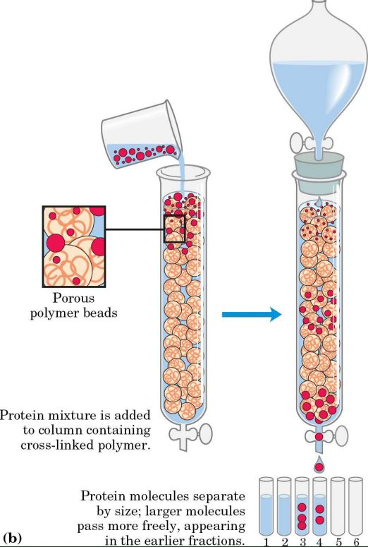
\includegraphics[width=.5\textwidth]{paste_src/2023-10-22-15-08-32.png}
\caption{分子篩管柱層析法}
\label{fig:mf}
\end{figure}


\section*{實驗步驟:}

\subsection*{實驗器材}

\begin{enumerate}[label=\arabic*.]
  \item 管柱、管柱夾
  \item 水
  \item 滴管
  \item 1xPBS緩衝液(Phosphate buffered Saline)
  \item Sephadex G-50 膠體懸浮液
  \item Sample:BSA(bovine serum albumin,牛血清蛋白)+ Methyl Orange
  \item	Eppendorf、Micropipette、ELISA plate
  \item	Bradford reagent
\end{enumerate}


\subsection*{步驟}

\begin{enumerate}[label=\arabic*.]
  \item 製備管柱
  \begin{enumerate}[label=(\arabic*)]
    \item 取管柱
  
    \item 加水進管柱,確定管柱可讓緩衝液順暢通過
    \item 塞住管柱
    \item 先加入 1xPBS 緩衝液到管柱中,並維持八分滿的高度
    \item 加入均質的 Sephadex G-50 膠體懸浮液
    \item 打開管柱
    \item 持續加入並使其沉降至黑線位置左右
    \item 滴管加 PBS 緩衝液進管柱,沖散 Sephadex G-50 使之重新均勻堆疊
    \item 待上方緩衝液流下,直到管柱下方不再滴出緩衝液就可以塞住管柱
  \end{enumerate}
  \item 放入Sample
  \begin{enumerate}[label=(\arabic*)]
    \item 用micropipette吸取10μl的BSA+Methyl orange(本次實驗 sample,BSA 濃度 50\mug/\mul)
    \item 將micropipette伸進管柱內,把Sample 滴加在膠體正上方(不可碰到管壁)
    \item 小心將緩衝液加入管柱內,需注意避免將Sample沖散,使緩衝液滿溢到管柱口,並形成表面張力。
  \end{enumerate}
  \item 收集樣品
  \begin{enumerate}[label=(\arabic*)]
    \item 將eppendorf事先標號碼。
    \item 打開管柱,馬上開始收集濾出來的液體。
    \item 每 10 滴收集到一個 eppendorf,共收集10管 (每一管大約350\mul)。
  \end{enumerate}
  \item 檢測收集成果並繪製雙曲線圖
  \begin{enumerate}[label=(\arabic*)]
    \item 利用 micropipette,分別將收集到的10個 eppendorf 取各取10μl,加入 100μl Bradford reagent,放在eppendorf中,在室溫中反應3$\sim$5分鐘,使其混合均勻。
    \item 取100μl放入ELISA plate,利用OD$_{595nm}$測定。此為確認大分子於何管柱流出。
    \item 另外取 100μl 未跟Bradford reagent 反應過的原樣品液,依序注入ELISA plate,利用OD$_{450nm}$測定。此為確認小分子於何管柱流出。
    \item 將結果繪製於excel檔中。
  \end{enumerate} 
  \item 測定純化出的大分子蛋白的濃度。
  \begin{enumerate}[label=(\arabic*)]
    \item 取OD$_{595nm}$吸光值最高的原始管子,進行Bradford assay。
    \item 取八支eppendorf,分別放入BSA 0,2,4,6,8,10μl及 A(2\mul unknown), B(2\mul unknown)溶於\ce{ddH2O}至最終容量為10μl。
    \begin{table}[ht]
      \centering
      \begin{tabular}{ccc}
      \toprule
      管號&BSA \ce{(\mu l)}& \ce{ddH2O(\mu l)}\\
      \midrule
      1&0&10\\
      2&2&8\\
      3&4&6\\
      4&6&4\\
      5&8&2\\
      6&10&0\\
      \midrule
      A (2μl Unknown)&2&8\\
      B (4μl Unknown)&4&6\\
    
      \bottomrule
    \end{tabular}\end{table}
    \item 每管加入 300μl 的 Bradford Reagent。
    \item 加入後,用手指輕彈eppendorf底部,並靜置5分鐘。
    \item 自八支eppendorf各吸取150\mul 至96孔盤。
    \item 放入ELISA reader,利用OD$_{595nm}$測定。
  \end{enumerate}

  
\end{enumerate}



\section*{實驗結果及討論:}
\subsection*{結果}
\begin{enumerate}
  \item 根據\prettyref{fig:gel_filtration},膠體過濾實驗中 OD$_{595nm}$(大分子蛋白質)的峰值發生在Fraction 3,而OD$_{450nm}$(小分子蛋白質)的峰值發生在Fraction 6。
  \item 根據\prettyref{tab:BSA}, \prettyref{fig:stand_curve} ,得知BSA濃度標準曲線 $y=0.0673x+0.0301,\ R^2=0.966$,即可推算 Fraction 3 的濃度為 0.804 \mug/\mul。 
  \item Fraction 3 的層析液約為 350\mul,而 Sample BSA 濃度為 50\mug/\mul 因此 BSA 回收率為
  $$
  \frac{0.804(\mug/\mul)\times 350(\mul)}{50(\mug/\mul)\times 10(\mul)}=0.562
  $$



\end{enumerate}


  




\subsection*{實驗數據}

\begin{table}[h]
\begin{minipage}[t]{0.45\textwidth}
  \setlength{\abovecaptionskip}{0cm} % 调整caption间距
  \caption{膠體層析吸光值數據}\label{tab:gel_filtration}
  \begin{tabular}{lll}
    \toprule
    fraction no.&OD$_{595nm}$&OD$_{450nm}$\\
    \midrule
    1&1.695&0.241\\
    2&1.767&0.204\\
    3&2.399&0.183\\
    4&0.953&0.226\\
    5&1.284&0.673\\
    6&1.196&0.818\\
    7&1.196&0.229\\
    8&1.481&0.198\\
    \bottomrule
  \end{tabular}
\end{minipage}
\begin{minipage}[t]{0.45\textwidth}
  \setlength{\abovecaptionskip}{0cm} % 调整caption间距
  \caption{BSA吸光值數據}\label{tab:BSA}
  \begin{tabular}{lll}
    \toprule
    BSA (mg)&OD$_{595nm}$&raw data\\
    \midrule
    0&0&0.759\\
    2&0.22&0.979\\
    4&0.328&1.087\\
    6&0.364&1.123\\
    8&0.552&1.311\\
    10&0.736&1.495\\
    \midrule
    A(2\mul\ unknown)&0.116&0.875\\
    B(4\mul\ unknown)&0.291&1.050\\
    \bottomrule
  \end{tabular}
\end{minipage}
\end{table}

\begin{table}[ht]
  \setlength{\abovecaptionskip}{0cm} % 调整caption间距
  \setlength{\tabcolsep}{10mm}{
  \caption{BAS吸光值回歸直線與回收率} \label{tab:result_data}
  \begin{tabular}{llll}
    \toprule
    y=a+bx&\\
    \midrule
    a&0.0673\\
    b&0.0301\\
    R$^2$&0.966\\
    \midrule
    A濃度&0.638 \mug/\mul\\
    B濃度&0.969 \mug/\mul\\
    平均濃度&0.804 \mug/\mul\\
    回收率&0.562\\
    \bottomrule
  \end{tabular}}
\end{table}

\subsection*{實驗作圖}

\begin{figure}[H]
\centering
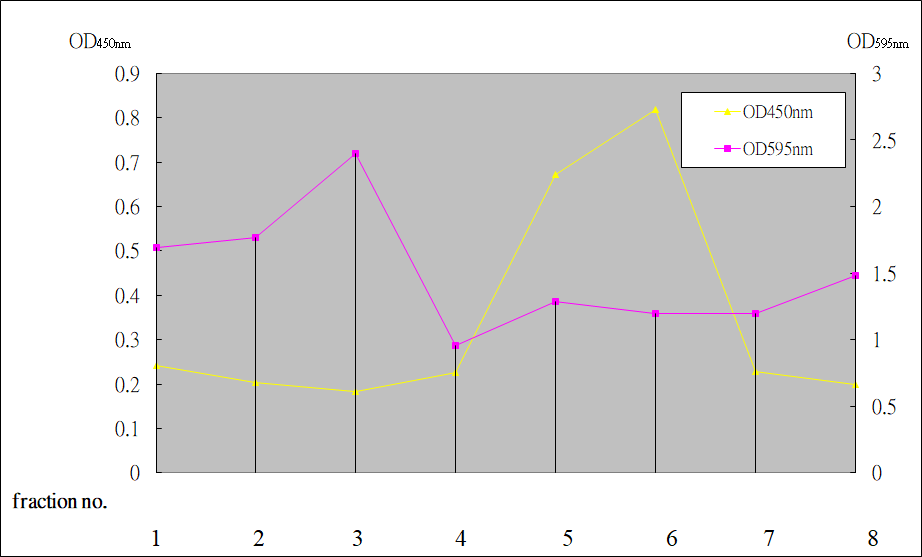
\includegraphics[width=.8\textwidth]{paste_src/2023-10-18-22-15-33.png}
\caption{膠體層析吸光值雙曲線}
\label{fig:gel_filtration}
\vspace{1em}
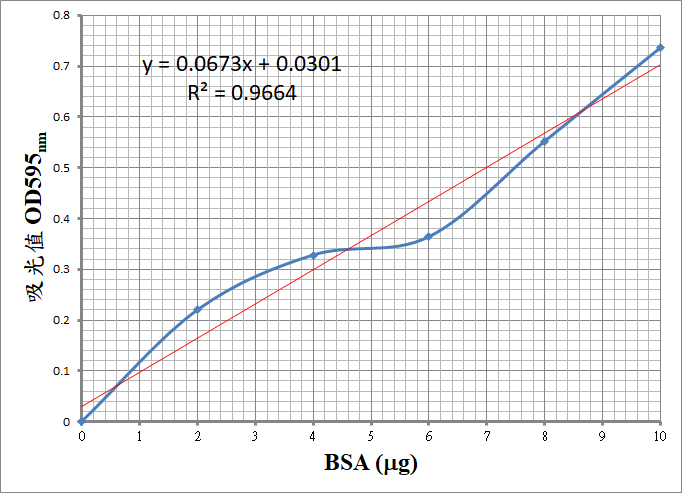
\includegraphics[width=.8\textwidth]{paste_src/2023-10-18-22-23-08.png}
\caption{BSA吸光值標準曲線}
\label{fig:stand_curve}
\end{figure}



\newpage
\subsection*{實驗討論:}
\begin{enumerate}[label=\arabic*.]
  \item 如\prettyref{tab:gel_filtration}, \prettyref{fig:gel_filtration},第一至第八管的順序為收集蛋白質的順序,可知第三管所收集到的大分子蛋白含量最高,第五和第六管則是收集到較多的小分子蛋白,因此可得出\textbf{小分子蛋白會在管柱內待得比較久}的結論。
  \item 老師上課有提到,兩個高峰值出現相距最好要超過兩管,才是比較好的分離,我們這次實驗大分子蛋白的峰值出現在第三管,小分子蛋白的峰值出現在第五及第六管,所以在分離方面有達到標準。
  \item BSA(大分子蛋白,\prettyref{fig:gel_filtration}中OD$_{595nm}$曲線)雖然第三管的峰值有做出來,但第一及第二管的數值偏高,造成此情況可能的原因是流速過快所導致。
  \item Methyl Orange(小分子蛋白,\prettyref{fig:gel_filtration}中OD$_{450nm}$曲線)峰值在第五及第六管,可能的原因為在放入Sample後,再加入緩衝液的力道過大,導致Sample有些微被沖散,因此離開管柱的時間拉長。
  \item \prettyref{fig:96}中E排為第一至第八管各取10\mul ,加入 100\mul\ Bradford reagent,已知 Bradford reagent 會與蛋白質結合呈現藍色。可以明顯以肉眼觀察到第三管有明顯的藍色,即第三管有最多的蛋白質。
  \item \prettyref{fig:96}圖中F排為第一至第八管各取100\mul,可以用肉眼觀察到第五及第六管明顯有收集到橘色的小分子蛋白(Methyl Orange)。
  \begin{figure}[H]
    \centering
    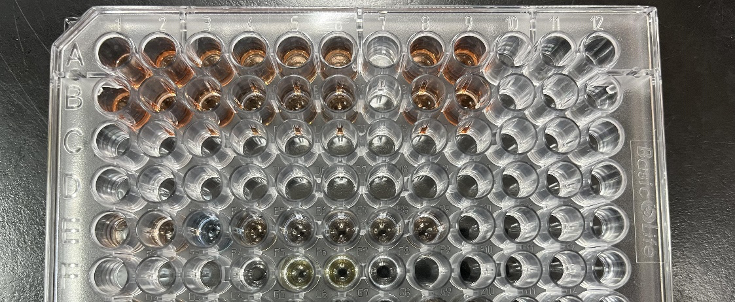
\includegraphics[width=.8\textwidth]{paste_src/2023-10-22-16-03-54.png}
    \caption{96孔盤}
    \label{fig:96}
  \end{figure}
  \item 蛋白質容液黏滯力較大,容易沾在 pipette tip 上導致 eppendorf 中 BSA 的量較少,ELISA 測出來的濃度偏低。而 \prettyref{tab:result_data} 中A管的濃度較B管低可能是因為 A 管的 BSA 量較少(2\mul),受到沾在 pipette tip 的蛋白質影響較大。我們仍需要加強 pipette 的使用技巧。
    
\end{enumerate}
  




\section{延伸討論}

\subsection*{Molecular Sieve(分子篩)}
Molecular Sieve(分子篩)是利用材料具有相似孔洞大小的特性,使小分子需要經過孔洞,所需要的時間較久,而大分子則會從孔洞旁經過,會較快經過材料,而達到分離不同大小分子的效果。IUPAC依據孔洞直徑的大小,將材料分為:\cite{Molecula6:online}%\url{https://en.wikipedia.org/wiki/Molecular_sieve}

\begin{itemize}
  \item Mircroporous material (<2nm)
  \item Mesoporous material (2nm~50nm)
  \item Macroporous material(>50nm)
\end{itemize}

然而更精確地來說,分離所依據的並非是分子的Molecular Weight,而是分子的Hydrodynamic Radius,所以就算是相同分子量的長鏈狀及球狀分子,其在分子篩管柱層析中的表現也不會一樣,球狀分子會需要比較久的時間才會析出。\cite{YMCSECMA7:online}
%https://ymctaiwan.com/portfolio/ymc_sec/#1607415269821-f456a30f-6b38






\bibliography{bibfile} 
\bibliographystyle{unsrt}


\end{document}
